\documentclass[12pt,a4paper]{article}
\usepackage[utf8]{inputenc}
\usepackage[spanish]{babel}
\usepackage{amsmath}
\usepackage{amsfonts}
\usepackage{amssymb}
\usepackage{graphicx}
\usepackage{kpfonts}
\usepackage[left=2cm,right=2cm,top=2cm,bottom=2cm]{geometry}
\title{EV 1-1 CIRCUITOS DE RECTIFICACIÓN NO CONTROLADOS}
\author{Sistemas electrónicos de interfaz\\
  \small Universidad Politécnica de la zona metropolitana de Guadalajara\\
\small Alan Antonio Muñoz Juárez\\
\small Giovanni Daniel Ruiz Tinoco\\
  \small 4-B \\
  \small Ing. Mecatrónica\\
\centering

\includegraphics[scale=2]{imagenes/p1.jpg} 
}

\begin{document}
\maketitle
\newpage
\section {Objetivo}
EL objetivo de esta práctica es realizar las simulaciones de los circuitos rectificadores no controlados para así analizar las funciones de onda resultantes.
\section {Materiales}
-Laptop\\
-Simulador de circuitos "KiCad"\\
\section {Procedimiento}
\subsection{Rectificador de media onda con carga inductiva}
Pese a que no es muy utilizado nos puede dar una referencia del comportamiento de un rectificador no controlado. En este caso usaremos el siguiente circuito
\\
\begin{center}
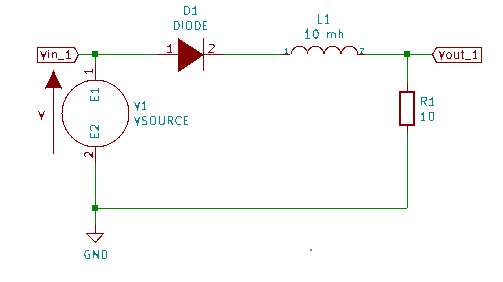
\includegraphics[scale=1]{imagenes/p1/C1.png} 
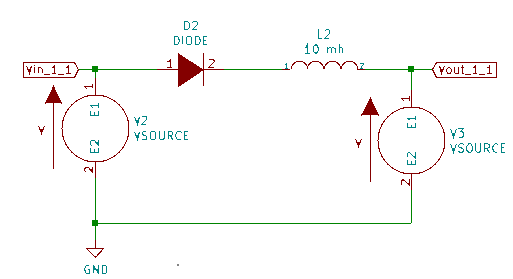
\includegraphics[scale=1]{imagenes/p1/C11.png} 
\end{center}
\begin{flushleft}
Como pondemos obsservar a continuación, vamos a analizar las ondas que este genera. 
\end{flushleft}
\begin{center}
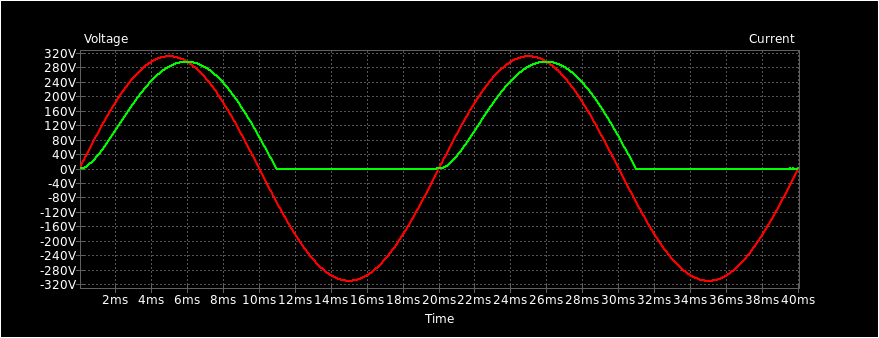
\includegraphics[scale=0.5]{imagenes/p1/P12.png} \\
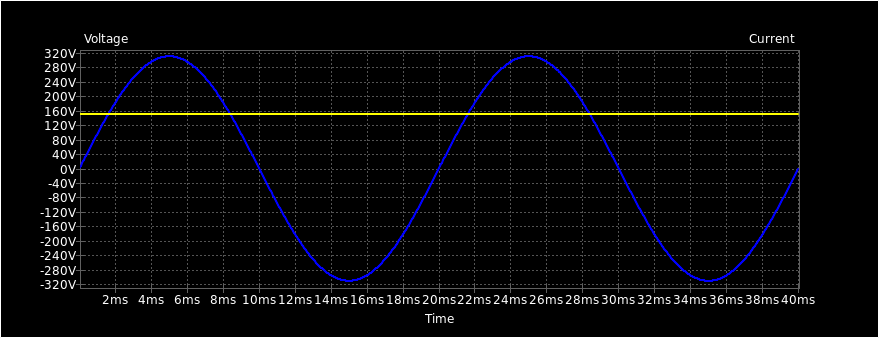
\includegraphics[scale=0.5]{imagenes/p1/P121.png} 
\end{center}
\subsection{Rectificador monofásico en puente}
\begin{flushleft}
Se muestra el siguiente esquema del rectificador monofásico en puente, La etapa de continua consta de un filtro constituido por los elementos Cf y Lf, destinado a atenuar el rizado de la tensión de salida. 
En la etapa de alterna se han añadido los elementos Rr y Lr para tener en cuenta, respectivamente, la resistencia y la inductancia de la red vistas desde el rectificador. 
\end{flushleft}
\begin{center}
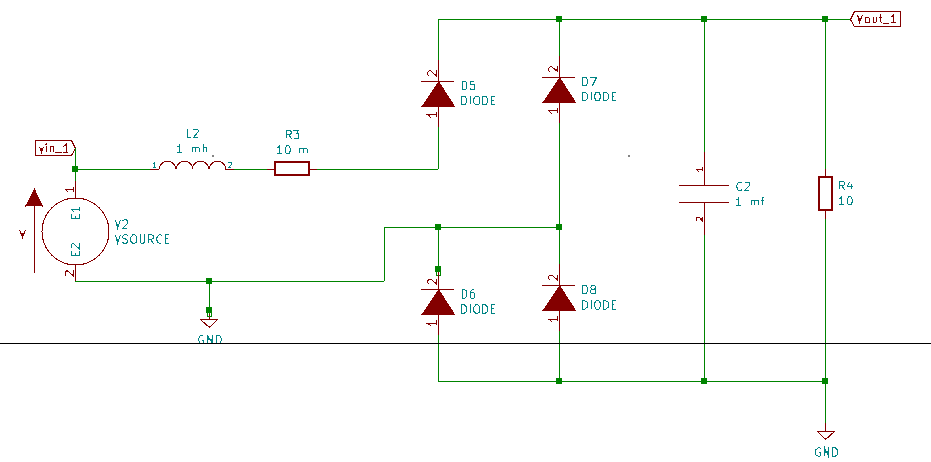
\includegraphics[scale=0.7]{imagenes/p2/Circuito2.png} 
\\ Al simular nuestro circuito sin modificar los parámetros, obtenemos la siguiente onda:\\
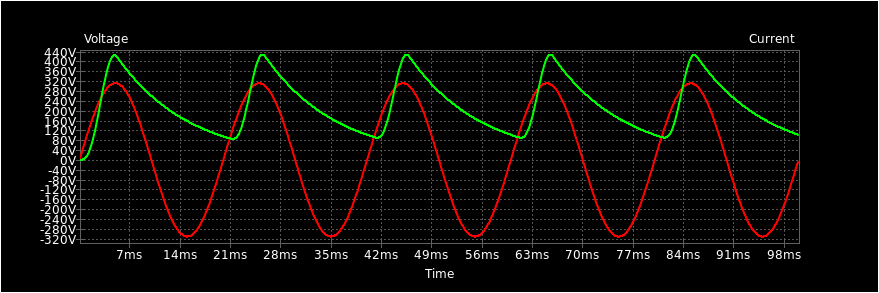
\includegraphics[scale=0.5]{imagenes/p2/practica131.png} 
 
En la siguiente imagen se muestra el efecto que tiene el capacitor sobre la corriente que pasa por los diodos\\
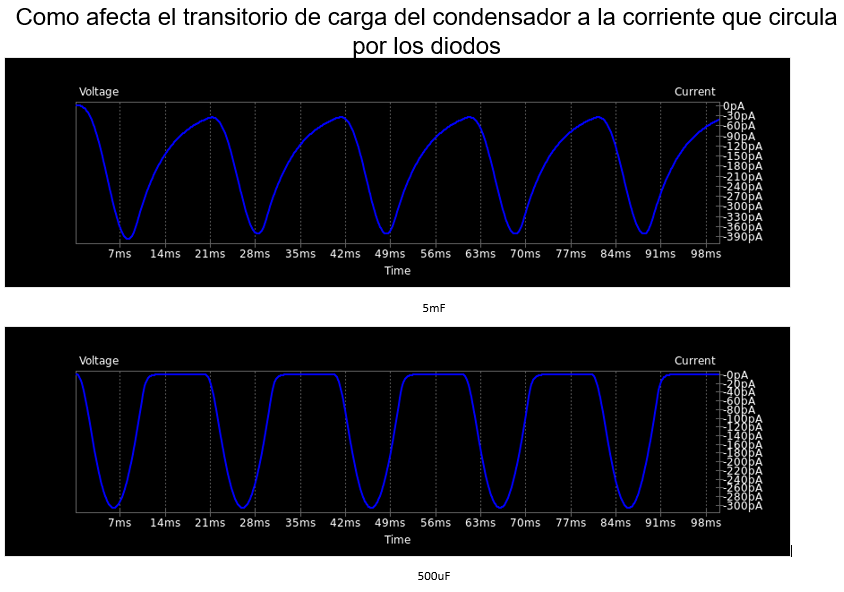
\includegraphics[scale=0.8]{imagenes/p2/dio3/diofinal.PNG} 
\\
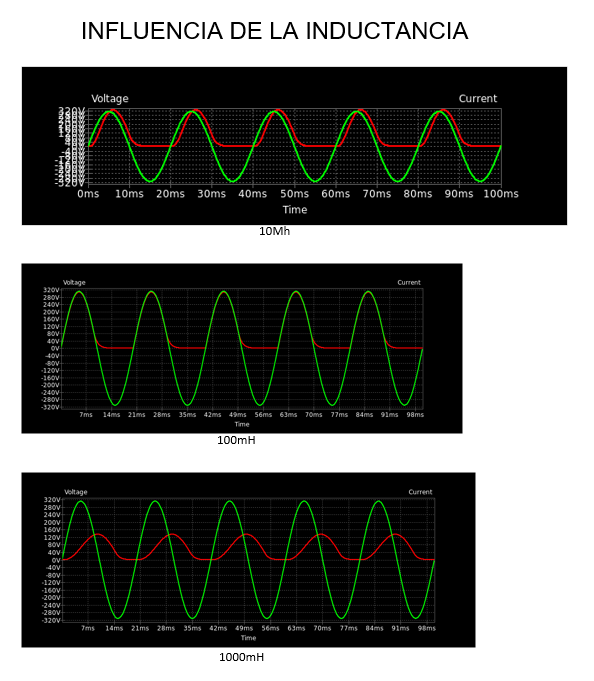
\includegraphics[scale=0.7]{imagenes/p2/inductor/induto.PNG} 
\\
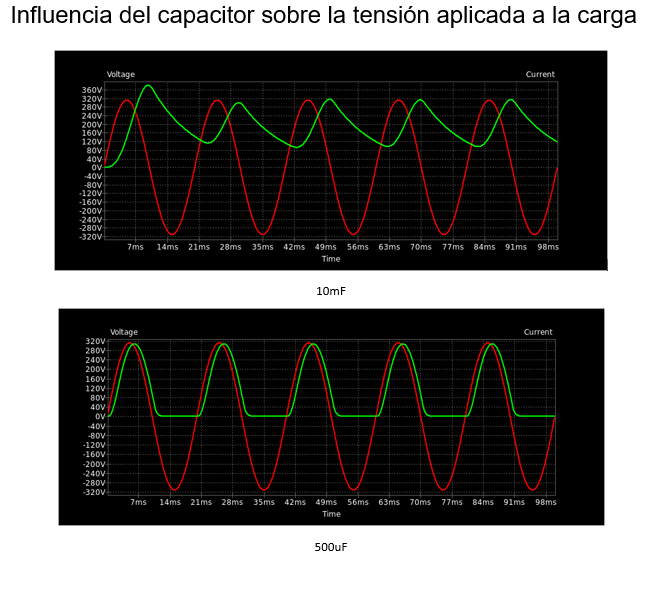
\includegraphics[scale=0.8]{imagenes/p2/caps/capfinal.PNG} 
\end{center}

\subsection{Rectificador monofásico de doble inductor}
\begin{flushleft}
Se tiene el siguiente circuito
\end{flushleft}
\begin{flushleft}
A continuación se muestra el circuito con el que vamos a trabajar:\\
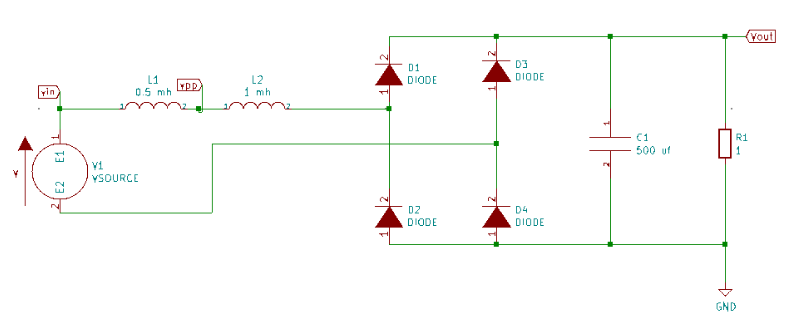
\includegraphics[scale=0.8]{imagenes/p3/Circuito3.png} 

Esta es la onda resultante de nuestro circuito sin modificar los parámetros:\\
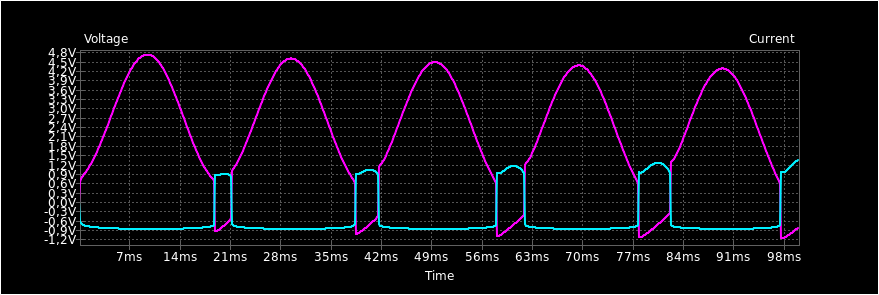
\includegraphics[scale=0.5]{imagenes/p3/practica12.png} 
\\
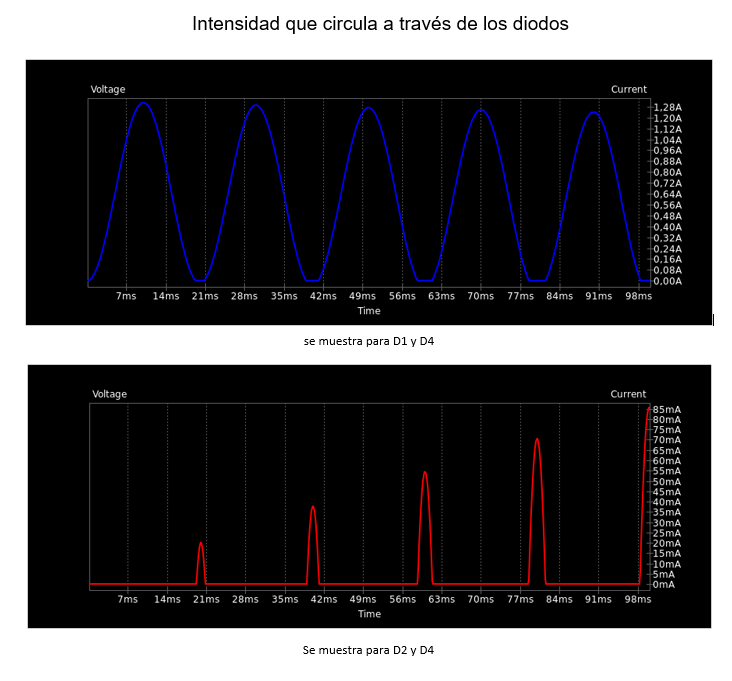
\includegraphics[scale=0.9]{imagenes/p3/dio/diofin.PNG} 
Vamos a armar el siguiente circuito
\newpage
En la siguiente imagen se puede apreciar como afecta el valor de la inductancia a la señal final del circuito:\\
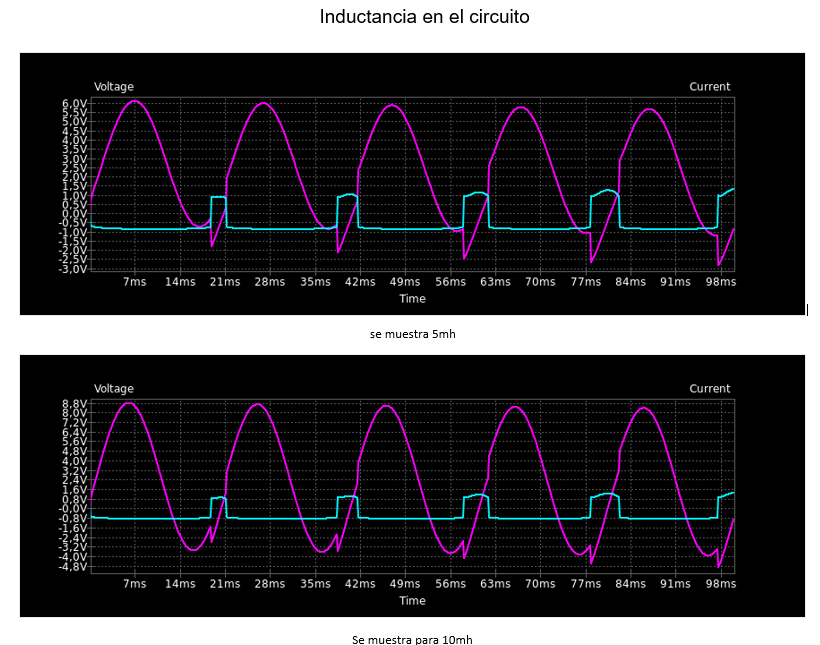
\includegraphics[scale=0.8]{imagenes/p3/lr/Inductanciafinal.PNG} 
\end{flushleft}
\newpage

\subsection{Rectificador monofásico duplicador de tensión}
\begin{flushleft}
Este tipo de rectificador, como su propio nombre indica, permite obtener en la salida una tensión que corresponde aproximadamente al doble de la que se obtiene con el circuito anterior.\\
De esta manera es posible obtener tensiones elevadas en la etapa de continua sin necesidad de utilizar un transformador que eleve la tension del rectificador.\\
\end{flushleft}
\begin{center}
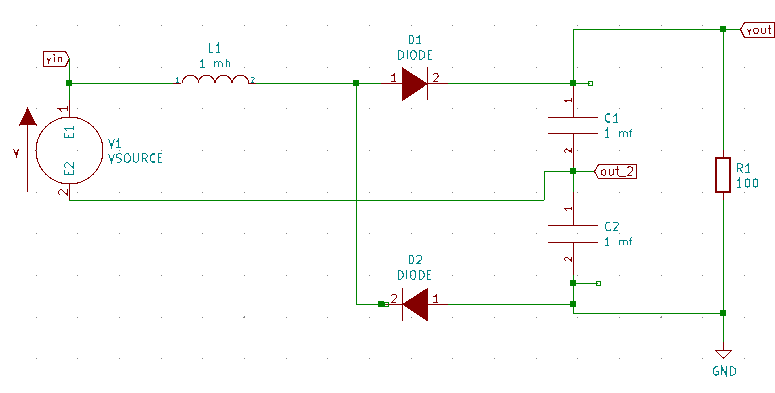
\includegraphics[scale=0.8]{imagenes/p4/Circuito4.png} 
\\
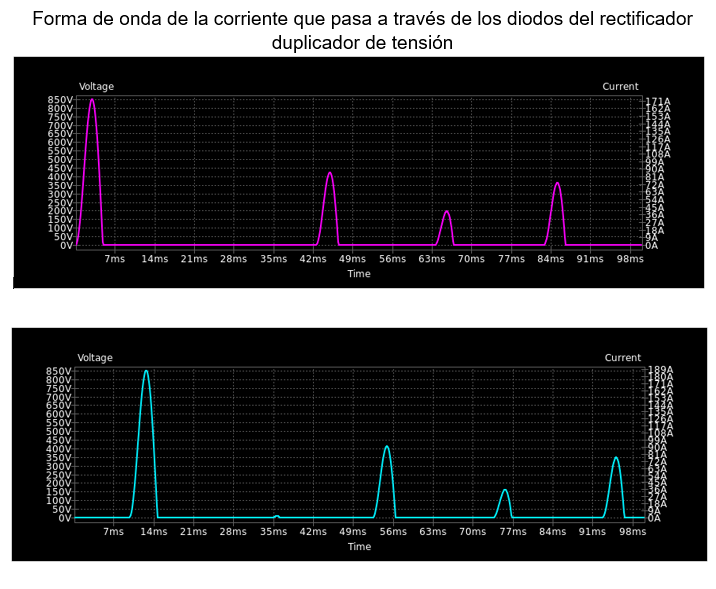
\includegraphics[scale=0.8]{imagenes/p4/dio/diodofinal.PNG} 
\end{center}

\subsection{Efectos de los rectificadores monofásicos en lineas trifásicas}
\begin{flushleft}
En epígrafes anteriores se ha puesto de manifiesgto algunos de los perjuicios que ocasionan los rectificadores monofásicos sobre las líneas de distribución que son:\\
1) Disminución del factor de potencia debido a la elevada distorsión armónica de la corriente.\\
2) Empobrecimiento de la calidad de la tensión en el punto común de conexión con los otros receptores
\\Este circuito se analizará por partes para ver como quedará finalmente.
En la primera parte podemos apreciar nuestro circuito
\begin{center}
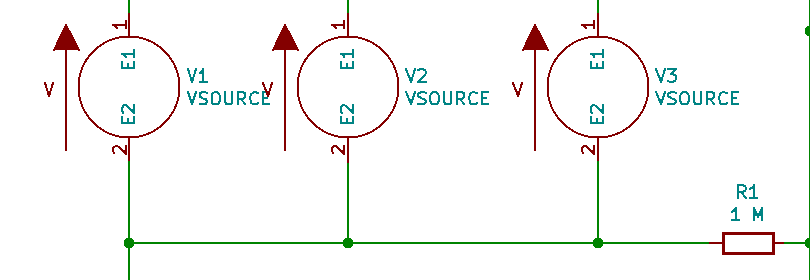
\includegraphics[scale=0.8]{imagenes/p5/Circuito4tri.png} \\
\end{center}
A continuación agregamos 3 veces este pequeño circuito el cual nos servirá para la rectificación de nuestra fuente trifásica:\\
\begin{center}
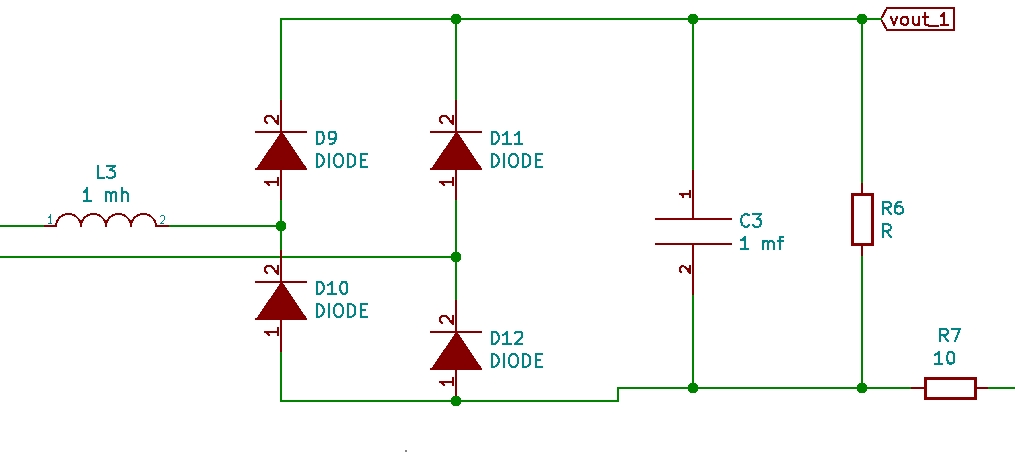
\includegraphics[scale=0.6]{imagenes/p5/Circuito4mono.png} \\
\end{center} 
\newpage
Nos quedará de la siguiente forma:\\
\begin{center}
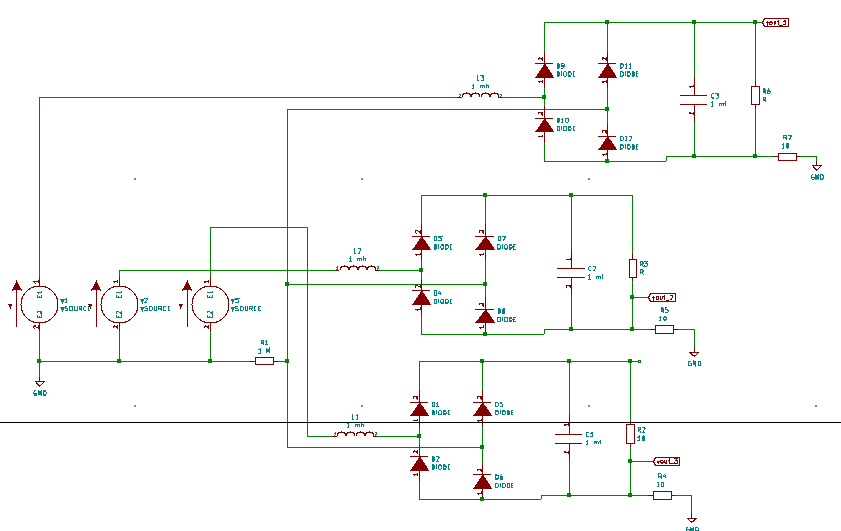
\includegraphics[scale=0.7]{imagenes/p5/Circuito4final.png} 
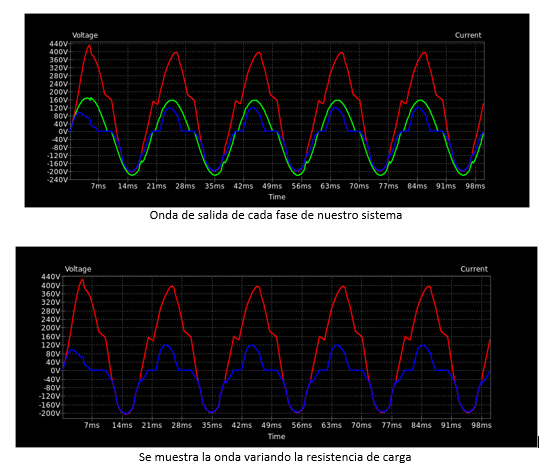
\includegraphics[scale=1]{imagenes/p5/simufinal.PNG} 
\end{center}
\end{flushleft}

\subsection{Rectificadores trifásicos}
\begin{flushleft}
Al igual que ocurre con el resto de receptores eléctricos, los circuitos rectificadores se utilizan en su versión trifásica cuando la potencia que consumen de la red es elevada, ya que en estos casos la utilización de rectificadores monofásicos provocarían desequilibrios importantes en el consumo de las fases. Este es el caso, entre otros ejemplos de la alimentacion de motores eléctricos de gran potencia, y la generación de redes de corriente continua.\\
\begin{center}
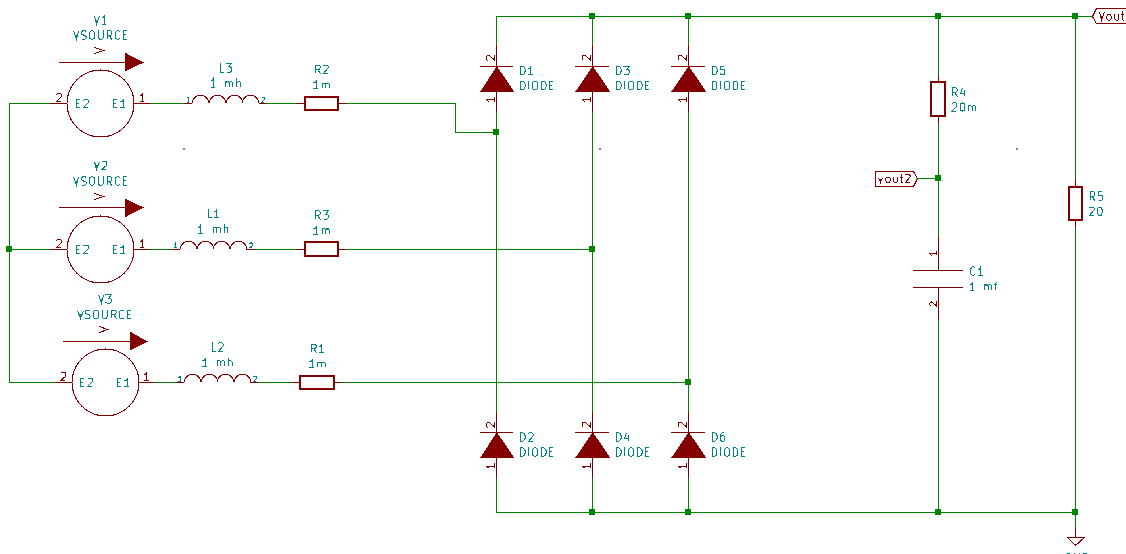
\includegraphics[scale=0.6]{imagenes/p6/Circuito6.png} 
\\
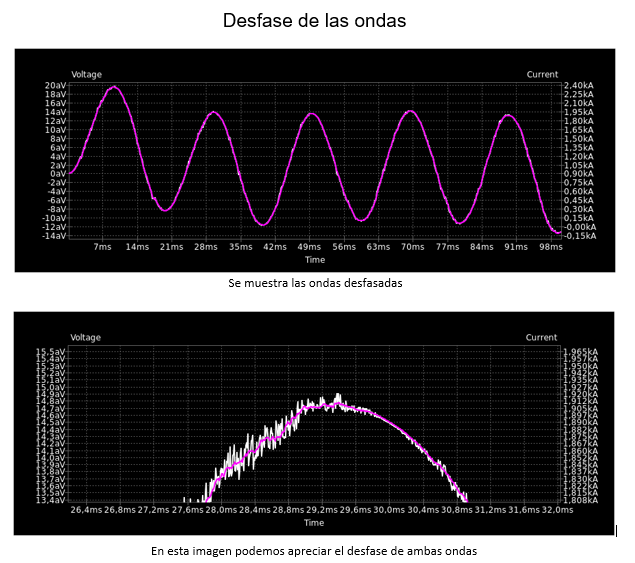
\includegraphics[scale=1]{imagenes/p6/desfase.PNG} 
\end{center}
\end{flushleft}
\newpage
\subsection{Efectos de las inductancias de red sobre la conmutación de corriente}
\begin{flushleft}
Cuando se añade un inductor de filtro en la etapa de continua, las inductancias de la línea provocan que la conmutación de corriente entre los diodos del rectiicador no sea instantánea. 
Para poner de manifiesto el fenómeno de la conmutación de corriente entre diodos y analizar sus efectos sobre el funcionamiento del rectificador, utilizaremos el circuito que aparece en la figura, en el que se modeliza la etapa de continua como una fuente de corriente constante.
\begin{center}
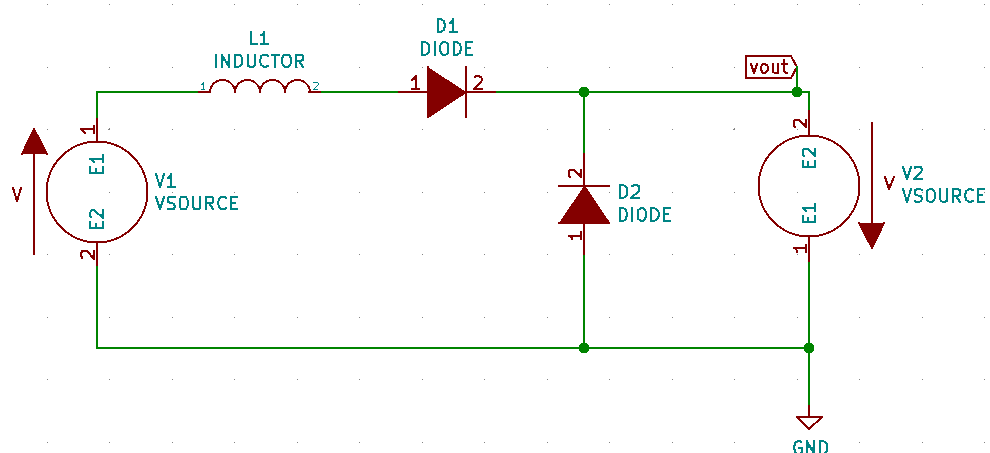
\includegraphics[scale=0.7]{imagenes/p7/Circuito7.png} 
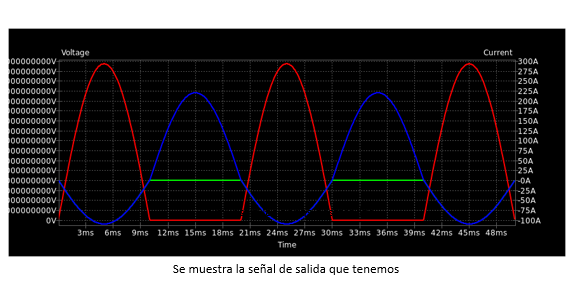
\includegraphics[scale=1]{imagenes/p7/onda.PNG} 
\end{center}
\end{flushleft}
\newpage
\section{Conclusiones}
\begin{flushleft}
En conclusión para los circuitos rectificadores confirmamos que para tensiones de entradas mucho mayores a la tensión directa del diodo (0.7v) el corrimiento se hace cada vez menos notorio. 
También se vertifica que al aumentar la capacitancia del capacitor, se logra una salida de corriente continua, también se presenta un alto rizado en las señales de salida, dicho rizado puede ser reducido al colocar un capacitor en paralelo a la carga.
\end{flushleft}
\end{document}

